\documentclass[twoside]{book}

% Packages required by doxygen
\usepackage{fixltx2e}
\usepackage{calc}
\usepackage{doxygen}
\usepackage[export]{adjustbox} % also loads graphicx
\usepackage{graphicx}
\usepackage[utf8]{inputenc}
\usepackage{makeidx}
\usepackage{multicol}
\usepackage{multirow}
\PassOptionsToPackage{warn}{textcomp}
\usepackage{textcomp}
\usepackage[nointegrals]{wasysym}
\usepackage[table]{xcolor}

% Font selection
\usepackage[T1]{fontenc}
\usepackage[scaled=.90]{helvet}
\usepackage{courier}
\usepackage{amssymb}
\usepackage{sectsty}
\renewcommand{\familydefault}{\sfdefault}
\allsectionsfont{%
  \fontseries{bc}\selectfont%
  \color{darkgray}%
}
\renewcommand{\DoxyLabelFont}{%
  \fontseries{bc}\selectfont%
  \color{darkgray}%
}
\newcommand{\+}{\discretionary{\mbox{\scriptsize$\hookleftarrow$}}{}{}}

% Page & text layout
\usepackage{geometry}
\geometry{%
  a4paper,%
  top=2.5cm,%
  bottom=2.5cm,%
  left=2.5cm,%
  right=2.5cm%
}
\tolerance=750
\hfuzz=15pt
\hbadness=750
\setlength{\emergencystretch}{15pt}
\setlength{\parindent}{0cm}
\setlength{\parskip}{0.2cm}
\makeatletter
\renewcommand{\paragraph}{%
  \@startsection{paragraph}{4}{0ex}{-1.0ex}{1.0ex}{%
    \normalfont\normalsize\bfseries\SS@parafont%
  }%
}
\renewcommand{\subparagraph}{%
  \@startsection{subparagraph}{5}{0ex}{-1.0ex}{1.0ex}{%
    \normalfont\normalsize\bfseries\SS@subparafont%
  }%
}
\makeatother

% Headers & footers
\usepackage{fancyhdr}
\pagestyle{fancyplain}
\fancyhead[LE]{\fancyplain{}{\bfseries\thepage}}
\fancyhead[CE]{\fancyplain{}{}}
\fancyhead[RE]{\fancyplain{}{\bfseries\leftmark}}
\fancyhead[LO]{\fancyplain{}{\bfseries\rightmark}}
\fancyhead[CO]{\fancyplain{}{}}
\fancyhead[RO]{\fancyplain{}{\bfseries\thepage}}
\fancyfoot[LE]{\fancyplain{}{}}
\fancyfoot[CE]{\fancyplain{}{}}
\fancyfoot[RE]{\fancyplain{}{\bfseries\scriptsize Generated on Thu Aug 4 2016 16\+:40\+:02 for Ser321 C++ Movie\+Client\+Gui by Doxygen }}
\fancyfoot[LO]{\fancyplain{}{\bfseries\scriptsize Generated on Thu Aug 4 2016 16\+:40\+:02 for Ser321 C++ Movie\+Client\+Gui by Doxygen }}
\fancyfoot[CO]{\fancyplain{}{}}
\fancyfoot[RO]{\fancyplain{}{}}
\renewcommand{\footrulewidth}{0.4pt}
\renewcommand{\chaptermark}[1]{%
  \markboth{#1}{}%
}
\renewcommand{\sectionmark}[1]{%
  \markright{\thesection\ #1}%
}

% Indices & bibliography
\usepackage{natbib}
\usepackage[titles]{tocloft}
\setcounter{tocdepth}{3}
\setcounter{secnumdepth}{5}
\makeindex

% Hyperlinks (required, but should be loaded last)
\usepackage{ifpdf}
\ifpdf
  \usepackage[pdftex,pagebackref=true]{hyperref}
\else
  \usepackage[ps2pdf,pagebackref=true]{hyperref}
\fi
\hypersetup{%
  colorlinks=true,%
  linkcolor=blue,%
  citecolor=blue,%
  unicode%
}

% Custom commands
\newcommand{\clearemptydoublepage}{%
  \newpage{\pagestyle{empty}\cleardoublepage}%
}


%===== C O N T E N T S =====

\begin{document}

% Titlepage & ToC
\hypersetup{pageanchor=false,
             bookmarks=true,
             bookmarksnumbered=true,
             pdfencoding=unicode
            }
\pagenumbering{roman}
\begin{titlepage}
\vspace*{7cm}
\begin{center}%
{\Large Ser321 C++ Movie\+Client\+Gui }\\
\vspace*{1cm}
{\large Generated by Doxygen 1.8.10}\\
\vspace*{0.5cm}
{\small Thu Aug 4 2016 16:40:02}\\
\end{center}
\end{titlepage}
\clearemptydoublepage
\tableofcontents
\clearemptydoublepage
\pagenumbering{arabic}
\hypersetup{pageanchor=true}

%--- Begin generated contents ---
\chapter{Hierarchical Index}
\section{Class Hierarchy}
This inheritance list is sorted roughly, but not completely, alphabetically\+:\begin{DoxyCompactList}
\item Fl\+\_\+\+Window\begin{DoxyCompactList}
\item \contentsline{section}{Movie\+Client\+Gui}{\pageref{class_movie_client_gui}}{}
\end{DoxyCompactList}
\end{DoxyCompactList}

\chapter{Class Index}
\section{Class List}
Here are the classes, structs, unions and interfaces with brief descriptions\+:\begin{DoxyCompactList}
\item\contentsline{section}{\hyperlink{class_movie_client_gui}{Movie\+Client\+Gui} }{\pageref{class_movie_client_gui}}{}
\end{DoxyCompactList}

\chapter{File Index}
\section{File List}
Here is a list of all documented files with brief descriptions\+:\begin{DoxyCompactList}
\item\contentsline{section}{src/cpp/\hyperlink{_movie_client_gui_8cpp}{Movie\+Client\+Gui.\+cpp} \\*Copyright (c) 2016 Tim Lindquist, Software Engineering, Arizona State University at the Polytechnic campus 

This program is free software; you can redistribute it and/or modify it under the terms of the G\+N\+U General Public License as published by the Free Software Foundation version 2 of the License }{\pageref{_movie_client_gui_8cpp}}{}
\end{DoxyCompactList}

\chapter{Class Documentation}
\hypertarget{class_movie_client_gui}{}\section{Movie\+Client\+Gui Class Reference}
\label{class_movie_client_gui}\index{Movie\+Client\+Gui@{Movie\+Client\+Gui}}
Inheritance diagram for Movie\+Client\+Gui\+:\begin{figure}[H]
\begin{center}
\leavevmode
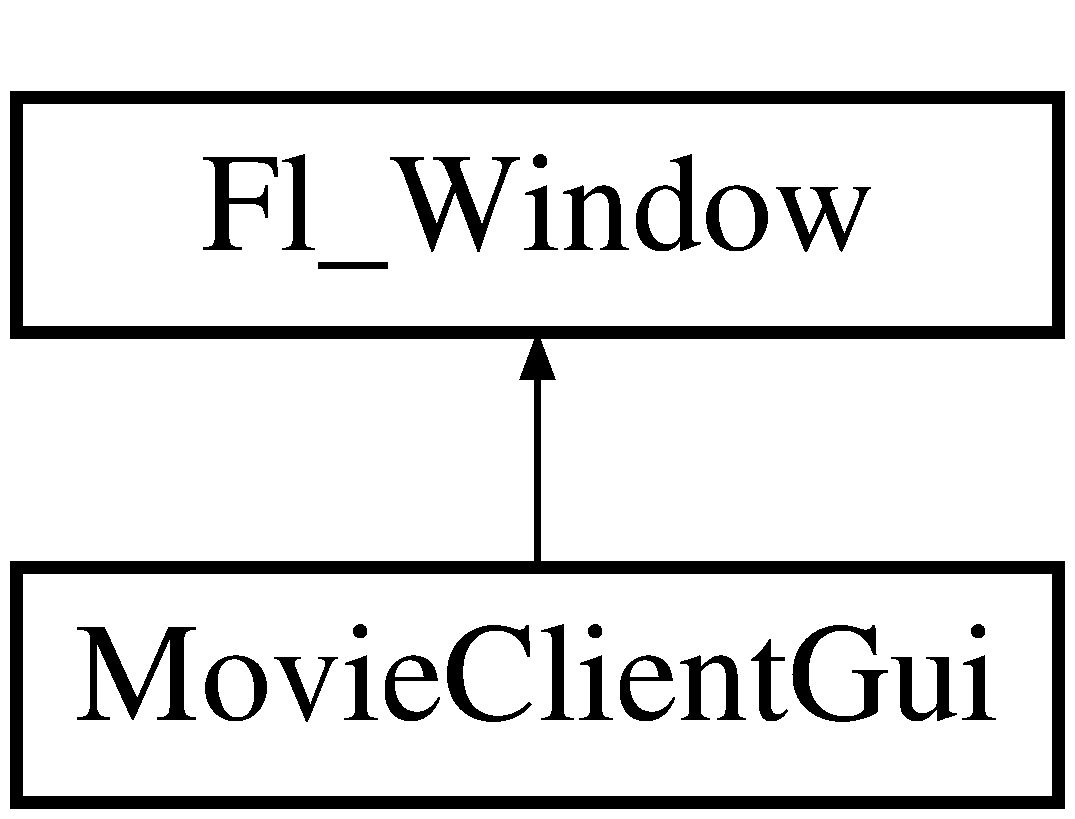
\includegraphics[height=2.000000cm]{class_movie_client_gui}
\end{center}
\end{figure}
\subsection*{Public Member Functions}
\begin{DoxyCompactItemize}
\item 
\hypertarget{class_movie_client_gui_a02ffc909104a55817d6608dfe35222f8}{}{\bfseries Movie\+Client\+Gui} (const char $\ast$name=\char`\"{}Ser321\char`\"{})\label{class_movie_client_gui_a02ffc909104a55817d6608dfe35222f8}

\end{DoxyCompactItemize}
\subsection*{Protected Attributes}
\begin{DoxyCompactItemize}
\item 
Fl\+\_\+\+Tree $\ast$ \hyperlink{class_movie_client_gui_af36267d1a841d6f1953abb2fd1549085}{tree}
\begin{DoxyCompactList}\small\item\em tree is the Fl\+\_\+\+Tree object that occupies the left side of the window. \end{DoxyCompactList}\item 
\hypertarget{class_movie_client_gui_a09459bc3627ba3f47a27df515d60eefb}{}Fl\+\_\+\+Input $\ast$ \hyperlink{class_movie_client_gui_a09459bc3627ba3f47a27df515d60eefb}{title\+Input}\label{class_movie_client_gui_a09459bc3627ba3f47a27df515d60eefb}

\begin{DoxyCompactList}\small\item\em title\+Input is the Fl\+\_\+\+Input object labelled Title Its for the user to enter the media tile (prefix filename). \end{DoxyCompactList}\item 
\hypertarget{class_movie_client_gui_a24100b71db9064b08ee16ba4ad2575ef}{}Fl\+\_\+\+Input $\ast$ \hyperlink{class_movie_client_gui_a24100b71db9064b08ee16ba4ad2575ef}{rated\+Input}\label{class_movie_client_gui_a24100b71db9064b08ee16ba4ad2575ef}

\begin{DoxyCompactList}\small\item\em rated\+Input is the Fl\+\_\+\+Input object labelled Rated Its for the user to enter the movie rating for videos \end{DoxyCompactList}\item 
\hypertarget{class_movie_client_gui_a612096ff4b484ca727cc6fbbb6e26526}{}Fl\+\_\+\+Input $\ast$ \hyperlink{class_movie_client_gui_a612096ff4b484ca727cc6fbbb6e26526}{runtime\+Input}\label{class_movie_client_gui_a612096ff4b484ca727cc6fbbb6e26526}

\begin{DoxyCompactList}\small\item\em author\+Input is the Fl\+\_\+\+Input object labelled Artist Its for the user to enter the artist for music, or for entering the primary actor for videos. \end{DoxyCompactList}\item 
\hypertarget{class_movie_client_gui_ae7c496133749474d8b1f0c37935ef6ea}{}Fl\+\_\+\+Input $\ast$ \hyperlink{class_movie_client_gui_ae7c496133749474d8b1f0c37935ef6ea}{released\+Input}\label{class_movie_client_gui_ae7c496133749474d8b1f0c37935ef6ea}

\begin{DoxyCompactList}\small\item\em released\+Input is the Fl\+\_\+\+Input object labelled Released Its for the user to enter the released date for videos. \end{DoxyCompactList}\item 
\hypertarget{class_movie_client_gui_a57815f6e0a5d6b57e88f252fe3c88d6c}{}Fl\+\_\+\+Input $\ast$ \hyperlink{class_movie_client_gui_a57815f6e0a5d6b57e88f252fe3c88d6c}{filename\+Input}\label{class_movie_client_gui_a57815f6e0a5d6b57e88f252fe3c88d6c}

\begin{DoxyCompactList}\small\item\em released\+Input is the Fl\+\_\+\+Input object labelled Released Its for the user to enter the released date for videos. \end{DoxyCompactList}\item 
\hypertarget{class_movie_client_gui_a13b2a12e2dc8a12f97f39d07cea98de4}{}Fl\+\_\+\+Multiline\+\_\+\+Input $\ast$ \hyperlink{class_movie_client_gui_a13b2a12e2dc8a12f97f39d07cea98de4}{plot\+M\+L\+In}\label{class_movie_client_gui_a13b2a12e2dc8a12f97f39d07cea98de4}

\begin{DoxyCompactList}\small\item\em plot\+M\+L\+In is the Fl\+\_\+\+Multiline\+\_\+\+Input object labelled Plot Its for the user to enter the video\textquotesingle{}s story-\/line. \end{DoxyCompactList}\item 
Fl\+\_\+\+Menu\+\_\+\+Bar $\ast$ \hyperlink{class_movie_client_gui_a6b91d5aaf8cb97e4d8c6fee6013fa203}{menubar}
\begin{DoxyCompactList}\small\item\em menubar is the Fl\+\_\+\+Menu\+\_\+\+Bar object. \end{DoxyCompactList}\item 
Fl\+\_\+\+Choice $\ast$ \hyperlink{class_movie_client_gui_adbe9044856cfbf73c9b2e5afd5292020}{genre\+Choice}
\begin{DoxyCompactList}\small\item\em Genre is the Fl\+\_\+\+Choice object labelled Genre. \end{DoxyCompactList}\item 
Fl\+\_\+\+Choice $\ast$ \hyperlink{class_movie_client_gui_ad6d29ccb3c824b894638f2667cb1200d}{actors\+Choice}
\begin{DoxyCompactList}\small\item\em Actors is the Fl\+\_\+\+Choice object labelled Actors. \end{DoxyCompactList}\end{DoxyCompactItemize}


\subsection{Member Data Documentation}
\hypertarget{class_movie_client_gui_ad6d29ccb3c824b894638f2667cb1200d}{}\index{Movie\+Client\+Gui@{Movie\+Client\+Gui}!actors\+Choice@{actors\+Choice}}
\index{actors\+Choice@{actors\+Choice}!Movie\+Client\+Gui@{Movie\+Client\+Gui}}
\subsubsection[{actors\+Choice}]{\setlength{\rightskip}{0pt plus 5cm}Fl\+\_\+\+Choice$\ast$ Movie\+Client\+Gui\+::actors\+Choice\hspace{0.3cm}{\ttfamily [protected]}}\label{class_movie_client_gui_ad6d29ccb3c824b894638f2667cb1200d}


Actors is the Fl\+\_\+\+Choice object labelled Actors. 

It provides the ability to enter and select actors. \hypertarget{class_movie_client_gui_adbe9044856cfbf73c9b2e5afd5292020}{}\index{Movie\+Client\+Gui@{Movie\+Client\+Gui}!genre\+Choice@{genre\+Choice}}
\index{genre\+Choice@{genre\+Choice}!Movie\+Client\+Gui@{Movie\+Client\+Gui}}
\subsubsection[{genre\+Choice}]{\setlength{\rightskip}{0pt plus 5cm}Fl\+\_\+\+Choice$\ast$ Movie\+Client\+Gui\+::genre\+Choice\hspace{0.3cm}{\ttfamily [protected]}}\label{class_movie_client_gui_adbe9044856cfbf73c9b2e5afd5292020}


Genre is the Fl\+\_\+\+Choice object labelled Genre. 

It provides the ability to enter and select genre \hypertarget{class_movie_client_gui_a6b91d5aaf8cb97e4d8c6fee6013fa203}{}\index{Movie\+Client\+Gui@{Movie\+Client\+Gui}!menubar@{menubar}}
\index{menubar@{menubar}!Movie\+Client\+Gui@{Movie\+Client\+Gui}}
\subsubsection[{menubar}]{\setlength{\rightskip}{0pt plus 5cm}Fl\+\_\+\+Menu\+\_\+\+Bar$\ast$ Movie\+Client\+Gui\+::menubar\hspace{0.3cm}{\ttfamily [protected]}}\label{class_movie_client_gui_a6b91d5aaf8cb97e4d8c6fee6013fa203}


menubar is the Fl\+\_\+\+Menu\+\_\+\+Bar object. 

Its the container for menus. \hypertarget{class_movie_client_gui_af36267d1a841d6f1953abb2fd1549085}{}\index{Movie\+Client\+Gui@{Movie\+Client\+Gui}!tree@{tree}}
\index{tree@{tree}!Movie\+Client\+Gui@{Movie\+Client\+Gui}}
\subsubsection[{tree}]{\setlength{\rightskip}{0pt plus 5cm}Fl\+\_\+\+Tree$\ast$ Movie\+Client\+Gui\+::tree\hspace{0.3cm}{\ttfamily [protected]}}\label{class_movie_client_gui_af36267d1a841d6f1953abb2fd1549085}


tree is the Fl\+\_\+\+Tree object that occupies the left side of the window. 

this tree control provides the ability to add and remove items and to manipulate and query the tree when an exception occurs. 

The documentation for this class was generated from the following file\+:\begin{DoxyCompactItemize}
\item 
src/cpp/\hyperlink{_movie_client_gui_8cpp}{Movie\+Client\+Gui.\+cpp}\end{DoxyCompactItemize}

\chapter{File Documentation}
\hypertarget{_movie_client_gui_8cpp}{}\section{src/cpp/\+Movie\+Client\+Gui.cpp File Reference}
\label{_movie_client_gui_8cpp}\index{src/cpp/\+Movie\+Client\+Gui.\+cpp@{src/cpp/\+Movie\+Client\+Gui.\+cpp}}


Copyright (c) 2016 Tim Lindquist, Software Engineering, Arizona State University at the Polytechnic campus 

This program is free software; you can redistribute it and/or modify it under the terms of the G\+N\+U General Public License as published by the Free Software Foundation version 2 of the License.  


{\ttfamily \#include $<$F\+L/\+Fl.\+H$>$}\\*
{\ttfamily \#include $<$F\+L/\+Fl\+\_\+\+Window.\+H$>$}\\*
{\ttfamily \#include $<$F\+L/\+Fl\+\_\+\+Button.\+H$>$}\\*
{\ttfamily \#include $<$F\+L/\+Fl\+\_\+\+Output.\+H$>$}\\*
{\ttfamily \#include $<$F\+L/\+Fl\+\_\+\+Tree.\+H$>$}\\*
{\ttfamily \#include $<$F\+L/\+Fl\+\_\+\+Tree\+\_\+\+Item.\+H$>$}\\*
{\ttfamily \#include $<$F\+L/\+Fl\+\_\+\+Menu\+\_\+\+Bar.\+H$>$}\\*
{\ttfamily \#include $<$F\+L/\+Fl\+\_\+\+Choice.\+H$>$}\\*
{\ttfamily \#include $<$F\+L/\+Fl\+\_\+\+Text\+\_\+\+Display.\+H$>$}\\*
{\ttfamily \#include $<$F\+L/\+Fl\+\_\+\+Text\+\_\+\+Buffer.\+H$>$}\\*
{\ttfamily \#include $<$F\+L/\+Fl\+\_\+\+Multiline\+\_\+\+Input.\+H$>$}\\*
{\ttfamily \#include $<$stdio.\+h$>$}\\*
{\ttfamily \#include $<$iostream$>$}\\*
{\ttfamily \#include $<$stdlib.\+h$>$}\\*
\subsection*{Classes}
\begin{DoxyCompactItemize}
\item 
class \hyperlink{class_movie_client_gui}{Movie\+Client\+Gui}
\end{DoxyCompactItemize}


\subsection{Detailed Description}
Copyright (c) 2016 Tim Lindquist, Software Engineering, Arizona State University at the Polytechnic campus 

This program is free software; you can redistribute it and/or modify it under the terms of the G\+N\+U General Public License as published by the Free Software Foundation version 2 of the License. 

This program is distributed in the hope that it will be useful, but without any warranty or fitness for a particular purpose. 

Please review the G\+N\+U General Public License at\+: \href{http://www.gnu.org/licenses/gpl-2.0.html}{\tt http\+://www.\+gnu.\+org/licenses/gpl-\/2.\+0.\+html} see also\+: \href{https://www.gnu.org/licenses/gpl-faq.html}{\tt https\+://www.\+gnu.\+org/licenses/gpl-\/faq.\+html} so you are aware of the terms and your rights with regard to this software. Or, write to the Free Software Foundation, Inc., 51 Franklin Street, Fifth Floor, Boston, M\+A 02110-\/1301,U\+S\+A 

Purpose\+: C++ F\+L\+T\+K view class for Movie client. \hyperlink{class_movie_client_gui}{Movie\+Client\+Gui} is the view for media app. This class is extended by the client controller which is the Movie\+Client class. Movie\+Client defines the call-\/backs for U\+I controls. It contains sample control functions that respond to button clicks and tree selects. This software is meant to run on Debian Jesse Linux 

Ser321 Principles of Distributed Software Systems see \href{http://pooh.poly.asu.edu/Ser321}{\tt http\+://pooh.\+poly.\+asu.\+edu/\+Ser321} \begin{DoxyAuthor}{Author}
Tim Lindquist (\href{mailto:Tim.Lindquist@asu.edu}{\tt Tim.\+Lindquist@asu.\+edu}) C\+I\+D\+S\+E -\/ Software Engineering, I\+A\+F\+S\+E, A\+S\+U at the Polytechnic campus
\end{DoxyAuthor}
\begin{DoxyDate}{Date}
July, 2016 
\end{DoxyDate}

%--- End generated contents ---

% Index
\backmatter
\newpage
\phantomsection
\clearemptydoublepage
\addcontentsline{toc}{chapter}{Index}
\printindex

\end{document}
